\chapter{反三角函数}
本章将在反函数理论的指导下,研究正弦、余弦、正切、余切存在反函数的条件,并在这些条件之下逐一地建立它们的反函数,进而研究这些反函数的性质、计算和应用。

\section{关于反函数知识的回顾}
\begin{example}
    已知函数$f(x)=x^2\; (x<0)$
\begin{enumerate}[(1)]
    \item $f(x)$是否存在反函数?说明理由;
    \item 若存在,试求之,并画出反函数的图象。
\end{enumerate}
\end{example}

\begin{solution}
\begin{enumerate}[(1)]
\item $f(x)=x^2\; (x<0)$是从集合$A=(-\infty,0)$到集合$B=(0,+\infty)$上的一一映射所确定的函数(图4.1中虚线给出的函数)。所以,$f(x)$存在反函数。
\item 由$y=x^2$, $x<0$, $y>0$,解出
\[x=-\sqrt{y},\quad y>0\]
改用习惯字母后,得
\[y=-\sqrt{x},\quad x>0\]
$\therefore\quad f^{-1}(x)=-\sqrt{x},\quad x>0$.

利用$f^{-1}(x)$与$f(x)$的图象关于直线$y=x$对称,由$f(x)$的图象画出$f^{-1}(x)$的图象(图4.1)。
\end{enumerate}
\end{solution}

\begin{rmk}
    本例所体现出来的下列三点都属于反函数理论的重要组成部分:
\begin{enumerate}[(1)]
    \item 函数$f(x)$存在反函数的条件:$f$是从$A$到$B$上的一一映射;
    \item 求反函数的步骤:先求出$x=f^{-1}(y),\; y\in B$,再写成$y=f^{-1}(x),\; x\in B$;
    \item 画反函数图象的方法:根据$y=f(x)$与$y=f^{-1}(x)$图象关于直线$y=x$的对称性,利用$y=f(x)$的图象直接作出$y=f^{-1}(x)$的图象。
\end{enumerate}
\end{rmk}


\noindent
\begin{minipage}{.45\textwidth}
  \centering
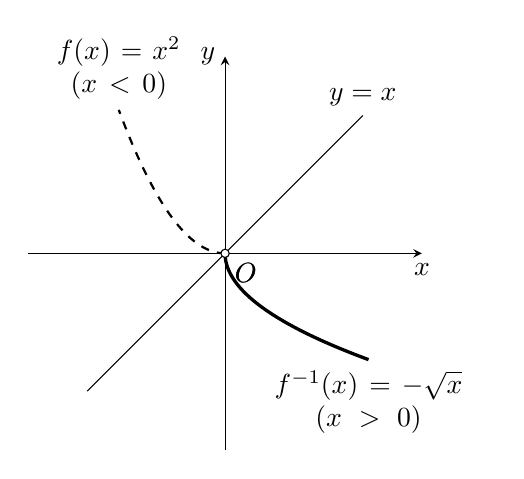
\begin{tikzpicture}[>=stealth]
\draw[->](-2.5,0)--(2.5,0)node[below]{$x$};
\draw[->](0,-2.5)--(0,2.5)node[left]{$y$};
\node [below right]{$O$};
\draw[domain=0:-1.35, smooth, dashed, thick]plot(\x, \x*\x)node[above, text width=2cm, align=center]{$f(x)=x^2$\\$(x<0)$};
\draw[domain=0:-1.35, smooth, very thick]plot(\x*\x, \x)node[below, text width=3cm, align=center]{$f^{-1}(x)=-\sqrt{x}$\\$(x>0)$};
\draw(-1.75,-1.75)--(1.75,1.75)node[above]{$y=x$};
\draw[fill=white](0,0)node[below right]{$O$} circle(1.5pt);

\end{tikzpicture}
\captionof{figure}{}
\end{minipage}
\hfill
\begin{minipage}{.45\textwidth}
  \centering
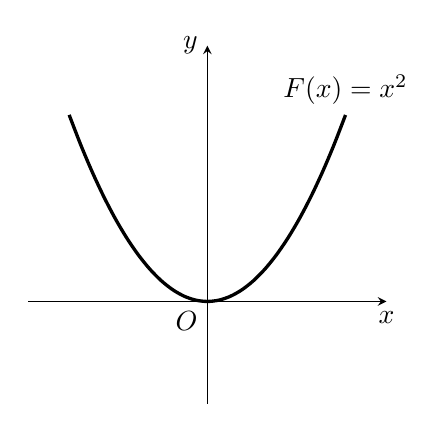
\begin{tikzpicture}[>=stealth, scale=1.3]
\draw[->](-1.75,0)--(1.75,0)node[below]{$x$};
\draw[->](0,-1)--(0,2.5)node[left]{$y$};
\node [below left]{$O$};
\draw[domain=-1.35:1.35, smooth, very thick]plot(\x, \x*\x)node[above]{$F(x)=x^2$};
\end{tikzpicture}
\captionof{figure}{}
\end{minipage}

\begin{thm}
 {问1} 函数$F(x)=x^2$, $x\in \R$存在反函数吗?   
\end{thm}

\begin{analyze}
    $F(x)$是从$A=(-\infty,+\infty)$到$B=[0,+\infty)$上的映射(图4.2),但不是一一映射(为什么?),所以$F(x)$不存在反函数。
\end{analyze}

\begin{thm}{问2 }
    对于上述$F(x)$,能否构造一个新的函数$f(x)$,使得
\begin{enumerate}
\item $f(x)$的定义域$A'$是$A$的子集;
   \item $f(x)$的对应法则与$F(x)$相同,即$f(x)=x^2,\; x\in A'$;
\item $f(x)$的值域仍为$B=[0,+\infty)$;
\item $f(x)$存在反函数。
\end{enumerate}
\end{thm}

\begin{analyze}
    从图4.2可以看出,只要取$A'=(-\infty,0]$或$A'=[0,+\infty)$都可以得到满足上述要求的新函数$f(x)$.
\end{analyze}

下面研究三角函数的反函数问题。根据一般函数的反函数的理论,自然会提出下面一些课题:
\begin{enumerate}[(1)]
\item 如何定义三角函数的反函数?
\item 三角函数的反函数的图象问题。
\item 三角函数的反函数有些什么性质?
\item 研究三角函数的反函数的基本方法。
\end{enumerate}

\section{反正弦函数}
\subsection{反正弦函数}

\begin{thm}
    {问1} $F(x):\; y=\sin x\; (x\in\R)$存在反函数吗?简述理由。
\end{thm}

\begin{thm}
{问2} 对于函数$F(x)$,能否找到$\R$的一个子集$A$,使得在$A$上得到的新函数
$f(x):\; y=\sin x,\; x\in A$, 其值域仍为$[-1,1]$,且$f(x)$存在反函数?    
\end{thm}

\begin{analyze}
 从正弦函数$y=\sin x\; (x\in\R)$显见,满足条件的子集$A$是很多的,如
\[\left[-\frac{\pi}{2},\; \frac{\pi}{2}\right],\; \left[\frac{\pi}{2},\; \frac{3\pi}{2}\right],\; \left[\frac{3\pi}{2},\; \frac{5\pi}{2}\right],\; \ldots\]
 总之,每一个$\left[-\frac{\pi}{2}+k\pi,\; \frac{\pi}{2}+k\pi\right]\; (k\in\Z)$都可以选作$A$。
\end{analyze}

在实际中,我们总是希望如上得到的$A$比较简单,而且包含所有锐角的值。这样选择$\left[-\frac{\pi}{2},\; \frac{\pi}{2}\right]=A$比较理想,即
\[f(x):\; y=\sin x,\quad x\in \left[-\frac{\pi}{2},\; \frac{\pi}{2}\right]\] 

\begin{thm}
    {思考题} 为什么说函数$f(x)$有反函数?
\end{thm}

\begin{thm}
{定义1} 函数$f(x):\; y=\sin x, \; x\in\left[-\frac{\pi}{2},\; \frac{\pi}{2}\right]$的反函
数称为\textbf{反正弦函数}\footnote{在英语中,“arc”一词表示弧,有的书上把反正弦函数写作$y=\sin^{-1}x$. 同样,后面讲到的反余弦函数、反正切函数、反余切函数也可写作$\cos^{-1}x$,$\tan^{-1}x$,$\cot^{-1} x$.},记为
\[f^{-1}(y):\; x=\arcsin y,\quad y\in[-1,1],\; x\in \left[-\frac{\pi}{2},\; \frac{\pi}{2}\right]\]    
\end{thm}

习惯上用字母$x$表示自变量,用$y$表示函数,所以要把$f^{-1}(y)$改写成
\[f^{-1}(x):\; y=\arcsin x,\quad x\in[-1,1],\; y\in \left[-\frac{\pi}{2},\; \frac{\pi}{2}\right]\]    

很明显,$f^{-1}$是从$B=[-1,1]$到$A=\left[-\frac{\pi}{2},\; \frac{\pi}{2}\right]$上的一一映射,它是$f:\; A\mapsto B$的逆映射。因此,对于$[-1,1]$中的每一个$x$值,$\arcsin x$表示唯一确定的角,这个角属于$\left[-\frac{\pi}{2},\; \frac{\pi}{2}\right]$,这个角的正弦恰好等于$x$。理解这一点,对研究反正弦函数的性质和运算至关重要。

\begin{example}
    求下列反正弦函数的值:
\begin{multicols}{2}
\begin{enumerate}[(1)]
    \item $\arcsin \frac{1}{2}$
    \item $\arcsin \left(-\frac{1}{2}\right)$
    \item $\arcsin \frac{\sqrt{2}}{2}$
    \item $\arcsin \left(-\frac{\sqrt{3}}{2}\right)$
    \item $\arcsin (-1)$
    \item $\arcsin 2$
\end{enumerate}
\end{multicols}
\end{example}

\begin{analyze}
这是已知正弦值,求在$\left[-\frac{\pi}{2},\; \frac{\pi}{2}\right]$上的角的问题.
\end{analyze}

\begin{solution}

\noindent
\begin{minipage}{.55\textwidth}
  \begin{enumerate}[(1)]
    \item 因为在$\left[-\frac{\pi}{2},\; \frac{\pi}{2}\right]$上,$\sin\frac{\pi}{6}=\frac{1}{2}$,所以
    \[\arcsin\frac{1}{2}=\frac{\pi}{6}\]
同理可得
\item $\arcsin \left(-\frac{1}{2}\right)=-\frac{\pi}{6}$
\item $\arcsin \frac{\sqrt{2}}{2}=\frac{\pi}{4}$
\item $\arcsin \left(-\frac{\sqrt{3}}{2}\right)=-\frac{\pi}{3}$
\item $\arcsin (-1)=-\frac{\pi}{2}$
\item 由于$2\notin [-1,1]$,所以$\arcsin 2$无意义.
\end{enumerate}
\end{minipage}
\hfill
\begin{minipage}{.4\textwidth}
  \centering
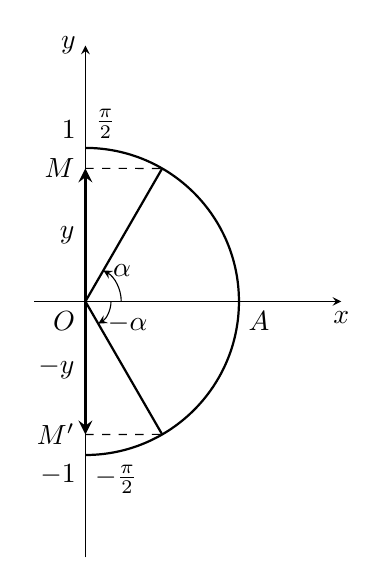
\begin{tikzpicture}[>=stealth, scale=1.3]
\draw[->](-.5,0)--(2.5,0)node[below]{$x$};
\draw[->](0,-2.5)--(0,2.5)node[left]{$y$};
\draw[thick](60:1.5)--(0,0)node [below left]{$O$}--(-60:1.5);
\draw[<->, very thick](0,1.3)node[left]{$M$}--node[left]{$y$}(0,0)--node[left]{$-y$}(0,-1.3)node[left]{$M'$};
\draw[thick](0,-1.5) arc (-90:90:1.5);
\node at (1.5,0)[below right]{$A$};
\draw[dashed](0,1.3)--(60:1.5);
\draw[dashed](0,-1.3)--(-60:1.5);
\node at (0,1.5)[above left]{1};
\node at (0,-1.5)[below left]{$-1$};
\node at (0,1.5)[above right]{$\frac{\pi}{2}$};
\node at (0,-1.5)[below right]{$-\frac{\pi}{2}$};
\draw[->](.35,0) arc (0:60:.35)node[right]{$\alpha$};
\draw[->](.25,0) arc (0:-60:.25)node[right]{$-\alpha$};
\end{tikzpicture}
\captionof{figure}{}
\end{minipage}


\end{solution}

\begin{remark}
    解这类求值题,联想正弦线的方向和大小是很有帮助的(图4.3)。也可结合反正弦函数的图象进行思考。下面研究反正弦函数的图象。
\end{remark}

\subsection{反正弦函数图象}
根据互为反函数的图象的性质,很自然想到,作函数$y=\sin x\; \left(-\frac{\pi}{2}\le x\le \frac{\pi}{2}\right) $的图象关于直线$y=x$的对称图形,便得到反正弦函数的图象(图4.4)。

\begin{figure}[htp]
    \centering
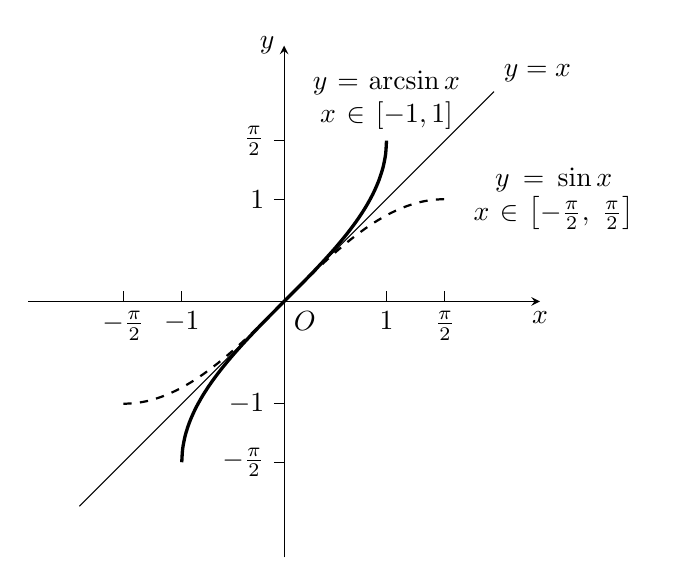
\begin{tikzpicture}[>=stealth, scale=1.3]
\draw[->](-2.5,0)--(2.5,0)node[below]{$x$};
\draw[->](0,-2.5)--(0,2.5)node[left]{$y$};
\foreach \x in {-1,1}
{
    \draw(\x,0)node[below]{$\x$}--(\x,.1);
    \draw(-.1,\x)node[left]{$\x$}--(0,\x);
    \draw(\x*pi/2,0)--(\x*pi/2,.1);
    \draw(-.1,\x*pi/2)--(0,\x*pi/2);
}
\node at (pi/2,0)[below]{$\frac{\pi}{2}$};
\node at (-pi/2,0)[below]{$-\frac{\pi}{2}$};
\node at (-.1,pi/2)[left]{$\frac{\pi}{2}$};
\node at (-.1,-pi/2)[left]{$-\frac{\pi}{2}$};
\node [below right]{$O$};
\draw(-2,-2)--(2.05,2.05)node[above right]{$y=x$};
\draw[domain=-0.5*pi:0.5*pi, smooth, dashed, thick]plot(\x, {sin(\x r)})node[right, text width=2.5cm, align=center]{$y=\sin x$\\ $x\in\left[-\frac{\pi}{2},\; \frac{\pi}{2}\right]$};
\draw[domain=-0.5*pi:0.5*pi, smooth, very thick]plot({sin(\x r)}, \x)node[above, text width=2.25cm, align=center]{$y=\arcsin x$\\ $x\in\left[-1, 1\right]$};
\end{tikzpicture}
    \caption{}
\end{figure}


\begin{thm}
    {思考题} 试观察反正弦函数的图象(图4.4),指出$y=\arcsin x$的定义域、值域,并研究其性质。
\end{thm}

\begin{example}
    求下列函数的定义域和值域:
\begin{multicols}{2}
\begin{enumerate}[(1)]
    \item $y=1-2\arcsin \frac{x}{3}$
    \item $y=\frac{1}{2}\arcsin(1-2x)$
\end{enumerate}
\end{multicols}
\end{example}

\begin{analyze}
用换元思想把所给问题转化为反正弦函数的问题加以解决,这是数学的基本方法。
\end{analyze}

\begin{solution}
\begin{enumerate}[(1)]
    \item $-1\le \frac{x}{3}\le 1\Longleftrightarrow -3\le x\le 3$

$\because\quad 2\arcsin\frac{x}{3}=1-y,\qquad \arcsin \frac{x}{3}=\frac{1}{2}(1-y)$

$\therefore\quad -\frac{\pi}{2}\le \frac{1}{2}(1-y)\le \frac{\pi}{2}$

$\therefore\quad -\pi-1\le -y\le \pi-1,\qquad 1-\pi\le y\le 1+\pi$

函数$y=1-2\arcsin \frac{x}{3}$的定义域是$[-3,3]$,值域是$[1-\pi,\; 1+\pi]$.

\item $-1\le 1-2x\le 1 \Longleftrightarrow -2\le -2x\le 0 \Longleftrightarrow 0\le x\le 1$

$\because\quad -\frac{\pi}{2}\le \arcsin(1-2x)\le \frac{\pi}{2}$

$\therefore\quad -\frac{\pi}{4}\le \frac{1}{2}\arcsin(1-2x)\le \frac{\pi}{4},\qquad -\frac{\pi}{4}\le y\le \frac{\pi}{4}$

函数$y=\frac{1}{2}\arcsin(1-2x)$的定义域是$[0,1]$,值域是$\left[-\frac{\pi}{4},\; \frac{\pi}{4}\right]$.
\end{enumerate}
\end{solution}

\subsection{反正弦函数的性质}

由于$\arcsin x$是$\left[-\frac{\pi}{2},\; \frac{\pi}{2}\right]$上的角,所以除特殊值外,
可以求其三角函数值。于是有下列问题:
\[\begin{split}
\sin(\arcsin x)=?&\qquad \cos(\arcsin x)=?\\
\tan(\arcsin x)=?&\qquad \cot(\arcsin x)=?    
\end{split}\]

同样,由于对任一$x\in[-1,1]$,$\arcsin x$都有唯一确定的值与之对应,那么,当用$\sin a$替换$\arcsin x$中的$x$,自然产生下面的问题:
\[\begin{split}
 \arcsin(\sin \alpha)=?&\qquad \arcsin(cos\alpha)=?\\
\arcsin(\tan\alpha)=? &\qquad \arcsin(\cot\alpha)=?\\
(\tan\alpha \in[-1,1]) &\qquad (\cot\alpha \in[-1,1]) 
\end{split} \]
根据反正弦函数的定义,参看图4.4或图4.3,不难得到关于\textbf{对应法则的基本公式}:
\begin{enumerate}[(1)]
    \item 当$x\in[-1,1]$时,$\sin(\arcsin x)=x$;当$x\ne [-1,1]$时,$\sin(\arcsin x)$无意义.
    \item 当$\alpha\in\left[-\frac{\pi}{2},\; \frac{\pi}{2}\right]$时,$\arcsin(\sin\alpha)=\alpha$;当$\alpha\notin\left[-\frac{\pi}{2},\; \frac{\pi}{2}\right]$时,$\arcsin(\sin\alpha)\ne \alpha$
\end{enumerate}

这里,当$\alpha\notin\left[-\frac{\pi}{2},\; \frac{\pi}{2}\right]$时,$\arcsin(\sin\alpha)\ne \alpha$是显而易见的. 例如,当$\alpha=\frac{5\pi}{6}$时,$\sin\frac{5\pi}{6}=\frac{1}{2}$,而
\[\arcsin\left(\sin\frac{5\pi}{6}\right)=\arcsin\frac{1}{2}=\frac{\pi}{6}\ne \frac{5\pi}{6}\]
从$\arcsin(\sin\alpha)\in \left[-\frac{\pi}{2},\; \frac{\pi}{2}\right]$也能判断$\arcsin\left(\sin\frac{5\pi}{6}\right)\ne \frac{5\pi}{6}$.

\begin{thm}{思考题}
$\alpha\notin  \left[-\frac{\pi}{2},\; \frac{\pi}{2}\right]$时,$\arcsin(\sin\alpha)=?$
\end{thm}

从图4.3或图4.4可以看出:
\begin{enumerate}[(1)]
\item 单调性:反正弦函数$y=\arcsin x$是$[-1,1]$上的增函数。
\item 奇偶性:反正弦函数$y=\arcsin x$是奇函数,即
\[\arcsin(-x)=-\arcsin x,\quad x\in[-1,1]\]
\end{enumerate}

\begin{example}
    求下列各式的值:
\begin{multicols}{2}
\begin{enumerate}[(1)]
    \item $\sin\left(\arcsin\frac{2}{3}\right)$
    \item $\sin\left[\arcsin\left(-\frac{1}{2}\right)\right]$
\end{enumerate}
\end{multicols}
\end{example}

\begin{solution}
\begin{enumerate}[(1)]
    \item $\because\quad \left|\frac{2}{3}\right|\le 1$\hfill (此步判断,十分必要)

$\therefore\quad \sin\left(\arcsin\frac{2}{3}\right)=\frac{2}{3}$

\item $\because\quad \left|-\frac{1}{2}\right|\le 1$

$\therefore\quad \sin\left[\arcsin\left(-\frac{1}{2}\right)\right]=-\frac{1}{2}$
\end{enumerate}
\end{solution}

\begin{example}
求下列各式的值:
\begin{multicols}{2}
\begin{enumerate}[(1)]
    \item $\tan\left(\arcsin \frac{\sqrt{3}}{2}\right)$
    \item $\cos\left[\arcsin \left(-\frac{2}{3}\right)\right]$
    \item $\cos\left(\arcsin x\right)$
    \item $\tan\left[\frac{1}{2}\arcsin\left(-\frac{1}{3}\right) \right]$
    \item $\cos\left(\arcsin\frac{1}{2}+\arcsin \frac{1}{3} \right)$
    \item $\tan\left(\arcsin\frac{2}{3}+\arcsin \frac{\sqrt{5}}{3}\right)$
\end{enumerate}
\end{multicols}
\end{example}

\begin{analyze}
 这是反正弦的三角运算。利用反正弦函数的定义或公式(1),是进行反正弦函数三角运算的基本方法。
\end{analyze}

\begin{solution}
\begin{enumerate}[(1)]
    \item $\tan\left(\arcsin \frac{\sqrt{3}}{2}\right)=tan\frac{\pi}{3}=\sqrt{3}$
    \item 设$t=\arcsin\left(-\frac{2}{3}\right)$,则$\sin t=-\frac{2}{3},\; t\in\left(-\frac{\pi}{2},0\right)$
\[\text{原式}=\cos t=\sqrt{1-\sin^2 t}=\sqrt{1-\left(-\frac{2}{3}\right)^2}=\frac{\sqrt{5}}{3}\]
\item 当$|x|>1$时,此式无意义.

当$|x|\le 1$时,设$t=\arcsin x$,则$\sin t=x,\; t\in\left[-\frac{\pi}{2},\; \frac{\pi}{2}\right]$
\[\text{原式}=\cos t=\sqrt{1-\sin^2 t}=\sqrt{1-x^2}\]

\item 设$t=\arcsin\left(-\frac{1}{3}\right)$,则
\[\begin{split}
    \sin t&=-\frac{1}{3},\quad t\in\left(-\frac{\pi}{2},\; 0\right)\\
    \cos t&=\sqrt{1-\sin^2 t}=\sqrt{1-\left(\frac{1}{3}\right)^2}=\frac{2\sqrt{2}}{3}
\end{split}\]
\[\text{原式}=\tan\frac{t}{2}=\frac{1-\cos t}{\sin t}=\frac{1-\frac{2\sqrt{2}}{3}}{-\frac{1}{3}}=2\sqrt{2}-3\]

\item 设$\alpha=\arcsin\frac{1}{2}$,$\beta=\arcsin\frac{1}{3}$,则
\[\begin{split}
    \alpha=\frac{\pi}{6},&\qquad \sin\alpha=\frac{1}{2},\qquad \cos\alpha=\frac{\sqrt{3}}{2}\\
    \sin\beta=\frac{1}{3},&\qquad \beta\in\left(0,\; \frac{\pi}{2}\right),\qquad \cos\beta=\frac{2\sqrt{2}}{3}
\end{split}\]
\[\begin{split}
    \text{原式}&=\cos(\alpha+\beta)=\cos\alpha\cos\beta-\sin\alpha\sin\beta\\
&=\frac{\sqrt{3}}{2}\x \frac{2\sqrt{2}}{3}-\frac{1}{2}\x\frac{1}{3}=\frac{2\sqrt{6}-1}{6}
\end{split}\]

\item 设$\alpha=\arcsin\frac{2}{3}$, $\beta=\arcsin\frac{\sqrt{5}}{3}$,则
\[\begin{split}
    \sin\alpha=\frac{2}{3},&\qquad \alpha\in\left(0,\frac{\pi}{2}\right),\qquad \tan\alpha=\frac{2}{\sqrt{5}}\\
    \sin\beta=\frac{\sqrt{5}}{3},&\qquad \beta\in\left(0,\frac{\pi}{2}\right),\qquad \tan\beta=\frac{\sqrt{5}}{2}
\end{split}\]
\[\text{原式}=\tan(\alpha+\beta)=\frac{\tan\alpha+\tan\beta}{1-\tan\alpha\tan\beta}\]

$\because\quad 1-\tan\alpha\tan\beta=1-\frac{2}{\sqrt{5}}\x \frac{\sqrt{5}}{2}=0$

$\therefore\quad $原式无意义.
\end{enumerate}
\end{solution}

\begin{example}
    求证:函数$y=\arcsin x$是$[-1,1]$上的增函数。
\end{example}

\begin{analyze}
    联想研究互为反函数的方法,此题利用公式(1), 借助于函数$y=\sin x$ $\left(-\frac{\pi}{2}\leq x\leq\frac{\pi}{2}\right)$的单调性证明。
\end{analyze}

\begin{proof}
    任取$x_1$、$x_2\in[-1,1]$, 且$x_1<x_2$,

    设$y_{1}= \arcsin x_{1}$, $y_{2}= \arcsin x_{2}$,
则 $x_{1}= \sin y_{1}$, $x_{2}= \sin y_{2}$, 且$y_1, y_{2}\in \left [ - \frac \pi 2, \;\frac \pi 2\right ] $

$\because\quad $在$\left[-\frac\pi2,\; \frac\pi2\right]$上正弦函数是增函数,假设$y_1\ge y_2$,
则$x_1\geqslant x_2$, 与$x_1<x_2$矛盾,

$\therefore y_{1}<y_{2}$,

$\therefore$ 函数$y=\arcsin x$是$[-1,1]$上的增函数。
\end{proof}

\begin{thm}
 {思考题} 试证$\arcsin(-x)=-\arcsin x$, $x\in[-1,1]$   
\end{thm}

\begin{example}
    求下列各式的值:
\begin{multicols}{2}
\begin{enumerate}[(1)]
    \item $\arcsin \left(\sin\frac{\pi}{5}\right)$
    \item $\arcsin \left(\sin\frac{4\pi}{7}\right)$
    \item $\arcsin \left[\sin\left(\frac{-338\pi}{3}\right)\right]$
    \item $\arcsin (\sin 8)$
\end{enumerate}
\end{multicols}
\end{example}

\begin{analyze}
 这是正弦的反正弦运算,利用公式(2)计算。此时,特别要判断角是否属于$\left[-\frac{\pi}{2},\; \frac{\pi}{2}\right]$
\end{analyze}

\begin{solution}
\begin{enumerate}[(1)]
    \item $\because\quad \frac{\pi}{5}\in \left[-\frac{\pi}{2},\; \frac{\pi}{2}\right]$
    
    $\therefore\quad \arcsin\left(\sin\frac{\pi}{5}\right)=\frac{\pi}{5}$

\item $\frac{4\pi}{7}\notin \left[-\frac{\pi}{2},\; \frac{\pi}{2}\right]$

$\because\quad \sin\frac{4\pi}{7}=\sin\frac{3\pi}{7},\quad \frac{3\pi}{7}\in \left[-\frac{\pi}{2},\; \frac{\pi}{2}\right]$

$\therefore\quad \arcsin\left(\sin\frac{4\pi}{7}\right)=\arcsin\left(\sin\frac{3\pi}{7}\right)=\frac{3\pi}{7}$
\item $-\frac{338\pi}{3}\notin \left[-\frac{\pi}{2},\; \frac{\pi}{2}\right]$

$\because\quad \sin\frac{-338\pi}{3}=\sin\left(112\pi-\frac{2\pi}{3}\right)=\sin\left(-\frac{2\pi}{3}\right)=\sin\left(-\frac{\pi}{3}\right)  $

$\therefore\quad \arcsin\left(\sin\frac{-338\pi}{3}\right)=\arcsin\left(\sin\frac{-\pi}{3}\right)=-\frac{\pi}{3}$

或$\because\quad \sin\frac{-338\pi}{3}=\sin\left(-\frac{2\pi}{3}\right)=-\sin\frac{2\pi}{3}=-\sin\frac{\pi}{3}$

$\therefore\quad \arcsin\left(\sin\frac{-338\pi}{3}\right)=\arcsin\left(-\sin\frac{\pi}{3}\right)=-\arcsin\left(\sin\frac{\pi}{3}\right)=-\frac{\pi}{3}$

\item $\because\quad 8\notin \left[-\frac{\pi}{2},\; \frac{\pi}{2}\right],\quad \frac{5\pi}{2}<8<3\pi$

$\therefore\quad \sin 8=\sin(3\pi-8),\quad 3\pi-8\in\left[-\frac{\pi}{2},\; \frac{\pi}{2}\right]$

$\therefore\quad \arcsin(\sin 8)=3\pi-8$
\end{enumerate}
\end{solution}

\begin{thm}
    {思考题}试求下面各式的值并探索一般方法:
\begin{multicols}{2}
\begin{enumerate}[(1)]
    \item $\arcsin\left(\cos\frac{4\pi}{5}\right)$
    \item $\arcsin\left[\tan\left(-\frac{\pi}{7}\right)\right] $
\end{enumerate}
\end{multicols}
\end{thm}

\section*{习题一}
\begin{center}
\bfseries A
\end{center}

\begin{enumerate}
    \item \begin{enumerate}[(1)]
        \item “$y=\arcsin x$的反函数是$y=\sin x$”这种说法对吗?为什么?
        \item $\arcsin(-\pi)$有意义吗?为什么?
        \item $\sin\left(\arcsin \frac{\pi}{5}\right)=\frac{\pi}{5}$能成立吗?为什么?
    \end{enumerate}
\item 求下列各式的值(可查表):
\begin{multicols}{2}
\begin{enumerate}[(1)]
    \item $\arcsin \frac{\sqrt{3}}{2}$
    \item $\arcsin \left(-\frac{\sqrt{2}}{2}\right)$
    \item $\arcsin 0$
    \item $\arcsin 1$
    \item $\arcsin \frac{\sqrt{6}+\sqrt{2}}{4}$
    \item $\arcsin\frac{\sqrt{6}-\sqrt{2}}{4}$
    \item $\arcsin 0.6959$
    \item $\arcsin \left(-\frac{1}{3}\right)$
\end{enumerate}
\end{multicols}

\item 求下列各式的值: 
\begin{multicols}{2}
\begin{enumerate}[(1)]
    \item $\sin \left(\arcsin \frac{4}{5}\right)$
    \item $\sin \left[\arcsin\left(-\frac{4}{5}\right)\right]$
    \item $\cos\left[\arcsin\left(-\frac{1}{2}\right)\right]$
    \item $\tan\left(\arcsin \frac{3}{5}\right) $
\end{enumerate}
\end{multicols}
\end{enumerate}

\begin{center}
    \bfseries B
\end{center}
\begin{enumerate}\setcounter{enumi}{3}
    \item 求下列函数的定义域和值域:
\begin{multicols}{2}
\begin{enumerate}[(1)]
    \item $y=\arcsin 2x$
    \item $y=\frac{1}{2}\arcsin x$
    \item $y=3\arcsin \frac{2x}{3}$
    \item $y=2\arcsin (1-x)$
\end{enumerate}
\end{multicols}
    \item 求下列各式的值: 
\begin{multicols}{2}
\begin{enumerate}[(1)]
    \item $\sin\left(2\arcsin\frac{1}{6}\right)$
    \item $\cos(2\arcsin 0.8)$
    \item $\tan\left(2\arcsin\frac{3}{4}\right)$
    \item $\sin\left[\frac{\pi}{3}+\arcsin\left(-\frac{1}{3}\right)\right]$
\end{enumerate}
\end{multicols}
    \item 求下列各式的值: 
\begin{multicols}{2}
\begin{enumerate}[(1)]
    \item $\arcsin \left(\sin\frac{3\pi}{4}\right)$
    \item $\arcsin \left[\sin\left(-\frac{3\pi}{4}\right)\right]$
    \item $\arcsin \left(\sin\frac{15\pi}{4}\right)$
    \item $\arcsin \left[\sin\left(-\frac{44\pi}{3}\right)\right]$
\end{enumerate}
\end{multicols}
    \item 求下列各式的值: 
\begin{multicols}{2}
\begin{enumerate}[(1)]
    \item $\tan(\arcsin x)$
    \item $\cos(2\arcsin x)$
    \item $\arcsin (\sin 5)$
    \item $\arcsin(\sin x),\quad x\in\left(\pi,\frac{3\pi}{2}\right)$
\end{enumerate}
\end{multicols}
\end{enumerate}

\section{反余弦函数}
类比反正弦函数研究的内容、程序和方法,试探索下面几个问题:
\begin{enumerate}[(1)]
\item 反余弦函数如何定义?
\item 反余弦函数图象如何画?
\item 反余弦函数有哪些性质?如何证明?
\item 研究和运用反余弦函数理论的基本方法是什么?应该注意哪些问题?
\end{enumerate}

在独立地得到结论后,再与下文做一对比.

1.反余弦函数的建立

函数$y=\cos x\; (x\in[0,\pi])$是从$[0,\pi]$到$[-1,1]$上的一一映射,因此,函数$y=\cos x$ $(x\in[0,\pi])$ 存在反函数。

\begin{thm}
    {定义2}函数$y=\cos x\; (x\in[0,\pi])$的反函数叫做反余弦函数,记作$y=\arccos x$,它的定义域是$[-1,1]$,它的值域是$[0,\pi]$.
\end{thm}

2.反余弦函数的图象

反余弦函数$y=\arccos x$的图象(如图4.5所示),它是与函数$y=\cos x$ $(x\in[0,\pi])$图象关于直线对称的图形。

\noindent
\begin{minipage}{.45\textwidth}
  \centering
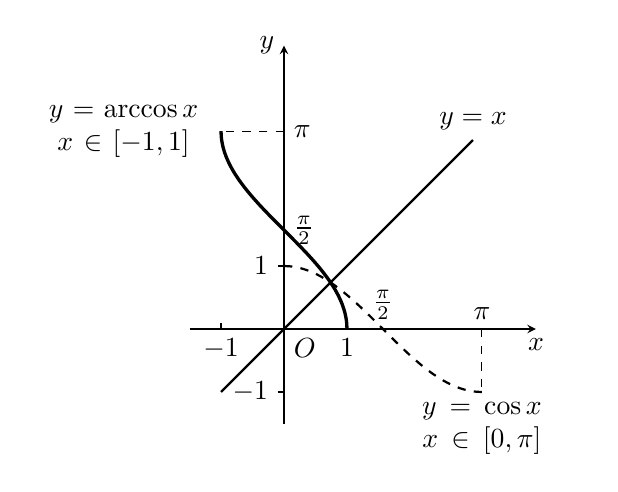
\begin{tikzpicture}[>=stealth, scale=.8]
\draw[->](-1.5,0)--(4,0)node[below]{$x$};
\draw[->](0,-1.5)--(0,4.5)node[left]{$y$};
\foreach \x in {-1,1}
{
    \draw(\x,.1)--(\x,0)node[below]{$\x$};
    \draw(-.1,\x)node[left]{$\x$}--(0,\x);
}
\draw[domain=0:pi, smooth, dashed, thick]plot(\x, {cos(\x r)})node[below, text width=2.5cm, align=center]{$y=\cos x$\\ $x\in[0,\pi]$};
\draw[domain=0:pi, smooth, very thick]plot({cos(\x r)}, \x )node[left, text width=2.2cm, align=center]{$y=\arccos x$\\ $x\in[-1,1]$};
\draw[dashed](pi,0)node[above]{$\pi$}--(pi,-1);
\draw[dashed](0,pi)node[right]{$\pi$}--(-1,pi);
\draw[thick](-1,-1)--(3,3)node[above]{$y=x$};
\node [below right]{$O$};
\node at (0.5*pi,0)[above]{$\frac{\pi}{2}$};
\node at (0,0.5*pi)[right]{$\frac{\pi}{2}$};


\end{tikzpicture}
\captionof{figure}{}
\end{minipage}
\hfill
\begin{minipage}{.45\textwidth}
  \centering
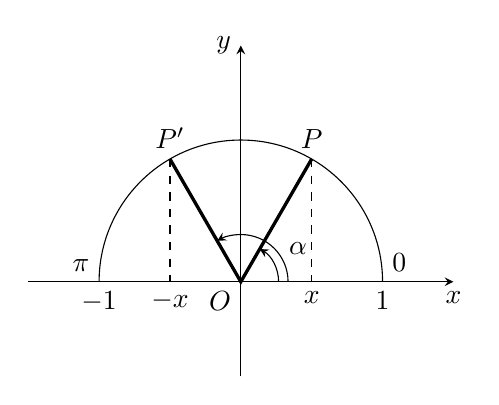
\begin{tikzpicture}[>=stealth, scale=1.2]
\draw[->](-2.25,0)--(2.25,0)node[below]{$x$};
\draw[->](0,-1)--(0,2.5)node[left]{$y$};
\draw(1.5,0)node[below]{1} arc (0:180:1.5)node[below]{$-1$};
\node at (1.5,0)[above right]{0};
\node at (-1.5,0)[above left]{$\pi$};
\draw[very thick](60:1.5)node[above]{$P$}--(0,0)--(120:1.5)node[above]{$P'$};
\draw[dashed](60:1.5)--(1.5/2,0)node[below]{$x$};
\draw[dashed](120:1.5)--(-1.5/2,0)node[below]{$-x$};
\node [below left]{$O$};
\draw[->](.4,0) arc (0:60:.4); 
\draw[->](.5,0) arc (0:120:.5); 
\node at (30:.7){$\alpha$};
\end{tikzpicture}
\captionof{figure}{}
\end{minipage}




3.反余弦函数的性质

根据反余弦函数的定义,参看图4.5或图4.6可以得到:
\begin{enumerate}[(1)]
    \item 对应法则的基本公式:
\begin{enumerate}
    \item 当$x\in[-1,1]$时,$\cos(\arccos x)=x$; 当$x\notin[-1,1]$时,$\cos(\arccos x)$无意义.
    \item  当$\alpha\in [0,\pi]$时,$\arccos(\cos\alpha)=\alpha$;当$\alpha\notin [0,\pi]$时,$\arccos(\cos\alpha)\ne \alpha$.
\end{enumerate}

\item 单调性:反余弦函数$y=\arccos x$是$[-1,1]$上的减函数。
\item 奇偶性:反余弦函数$y=\arccos x$是非奇非偶函数。而且有
\[\arccos(-x)=\pi-\arccos x,\quad x\in [-1,1]\]
\end{enumerate}

\begin{example}
    求证:$\arccos(-x)=\pi-\arccos x,\quad x\in [-1,1]$.
\end{example}

\begin{analyze}
    本题可以从反余弦函数定义出发,只需证明$π-\arccos x\in[0,\pi]$且其余弦值为$-x$即可。
\end{analyze}

\begin{proof}
   $\because\quad  x\in [-1,1],\qquad \therefore\quad -x\in [-1,1]$,

等式两边均有意义,
\[\cos(\pi-\arccos x)=-\cos(\arccos x)=-x\]
$\because\quad 0\le \arccos x\le \pi, \qquad \therefore\quad 0\ge -\arccos x\ge -\pi$
\[\pi\ge \pi-\arccos x\ge 0,\quad \text{即} 0\le \pi-\arccos x\le \pi\]

因此,$\pi-\arccos x$是属于$[0,\pi]$的角,且它的余弦等于$-x$,于是
\[\arccos(-x)=\pi-\arccos x\]
\end{proof}

\begin{example}
    求下列各式的值:
\begin{multicols}{2}
\begin{enumerate}[(1)]
    \item $\arccos \frac{\sqrt{3}}{2}$
    \item $\arccos \left(-\frac{\sqrt{2}}{2}\right)$
    \item $\arccos \left(\cos\frac{6\pi}{7}\right)$
    \item $\arccos \left[\cos\left(-\frac{46\pi}{5}\right)\right]$
    \item $\arccos (\cos 10)$
    \item $\arccos (\cos x),\quad x\in\left(-\frac{\pi}{2},0\right)$
\end{enumerate}
\end{multicols}
 \end{example}   


\begin{analyze}
后四小题是余弦的反余弦运算,应用公式(2)去做,解题时应判断角是否属于$[0,\pi]$。
\end{analyze}

\begin{solution}
\begin{enumerate}[(1)]
    \item $\because\quad$在$[0,\pi]$上,$\cos\frac{\pi}{6}=\frac{\sqrt{3}}{2}$

$\therefore\quad \arccos\frac{\sqrt{3}}{2}=\frac{\pi}{6}$

\item $\because\quad$在$[0,\pi]$上,$\cos\frac{3\pi}{4}=-\frac{\sqrt{2}}{2}$

$\therefore\quad \arccos\left(\frac{\sqrt{2}}{2}\right)=\frac{3\pi}{4}$

或
\[\arccos\left(\frac{\sqrt{2}}{2}\right)=\pi-\arccos\frac{\sqrt{2}}{2}=\pi-\frac{\pi}{4}=\frac{3\pi}{4}\]

\item $\because\quad \frac{6\pi}{7}\in [0,\pi]$

$\therefore\quad \arccos\left(\cos\frac{6\pi}{7}\right)=\frac{6\pi}{7}$

\item 由于$-\frac{46\pi}{5}\notin [0,\pi]$,而$-\frac{46\pi}{5}=-10\pi+\frac{4\pi}{5}$

$\therefore\quad \cos\left(-\frac{46\pi}{5}\right)=\cos\left(-10\pi+\frac{4\pi}{5}\right)=\cos\frac{4\pi}{5}$

$\because\quad \frac{4\pi}{5}\in[0,\pi]$
    
$\therefore\quad \arccos\left[\cos\left(-\frac{46\pi}{5}\right)\right]=\arccos\left(\cos\frac{4\pi}{5}\right)=\frac{4\pi}{5}$
    
\item 由于$10\notin [0,\pi]$,而$3\pi<10<4\pi$

$\therefore\quad 0<4\pi-10<\pi$

$\because\quad \cos10=\cos(-10)=\cos(4\pi-10)$

$\therefore\quad \arccos(\cos 10)=\arccos[\cos(4\pi-10)]=4\pi-10$

\item $\because\quad x\in\left(-\frac{\pi}{2},0\right)\qquad \therefore\quad -x\in\left(0,\frac{\pi}{2}\right)$

$\because\quad \cos x=\cos(-x)$

$\therefore\quad \arccos(\cos x)=\arccos[\cos(-x)]=-x$.
\end{enumerate}    
\end{solution}


\begin{example}
求下列各式的值:
\begin{multicols}{2}
\begin{enumerate}[(1)]
    \item $\cos\left[\arccos \left(-\frac{2}{3}\right)\right]$
    \item $\sin\left[\arccos \left(-\frac{4}{5}\right)\right]$
    \item $\tan(\arccos x)$
    \item $\cos\left[\arccos\frac{4}{5}+\arccos\left(-\frac{5}{13}\right)\right]$
\end{enumerate}    
\end{multicols}
\end{example}

\begin{analyze}
这是反余弦的三角运算问题。利用反余弦函数定义或公式(1),转化为三角函数问题进行计算。
\end{analyze}

\begin{solution}
\begin{enumerate}[(1)]
    \item $\because\quad \left[-\frac{2}{3}\right]\le 1$

$\therefore\quad \cos\left[\arccos\left(-\frac{2}{3}\right)\right]=-\frac{2}{3}$

\item 设$\alpha=\arccos\left(-\frac{4}{5}\right)$,则$\cos\alpha=-\frac{4}{5},\; \alpha\in[0,\pi]$

$\therefore\quad \sin\alpha=\sqrt{1-\cos^2\alpha}=\sqrt{1-\left(-\frac{4}{5}\right)^2}=\frac{3}{5}$

$\therefore\quad \sin\left[\arccos\left(-\frac{4}{5}\right)\right]=\frac{3}{5}$

\item 当$|x|>1$时,$\arccos x$无意义,原式无意义;当$|x|\le 1$且$x\ne 0$时,由$\arccos x\in[0,\pi]$,知$\sin(\arccos x)\ge 0$

$\therefore\quad \tan(\arccos x)=\frac{\sin(\arccos x)}{\cos(\arccos x)}=\frac{\sqrt{1-[\cos(\arccos x)]^2}}{\cos(\arccos x)}=\frac{\sqrt{1-x^2}}{x}$

当$x=0$时,$\arccos 0=\frac{\pi}{2}$,$\tan(\arccos x)$无意义.

\item 设$\alpha=\arccos \frac{4}{5}$,$\beta=\arccos\left(-\frac{5}{13}\right)$,则:
\[\begin{split}
    \cos\alpha=\frac{4}{5},&\qquad \alpha\in[0,\pi],\qquad \sin\alpha=\frac{3}{5}\\
    \cos\beta=-\frac{5}{13} ,&\qquad \beta\in[0,\pi],\qquad \sin\beta=\frac{12}{13}
\end{split}\]
\[\begin{split}
    \therefore\quad \text{原式}&=\cos(\alpha+\beta)=\cos\alpha\cos\beta-\sin\alpha\sin\beta\\
    &=\frac{4}{5}\x\left(-\frac{5}{13}\right)-\frac{3}{5}\x\frac{12}{13}=-\frac{56}{65}
\end{split}\]
\end{enumerate}
\end{solution}

\section*{习题二}
\begin{center}
\bfseries A
\end{center}

\begin{enumerate}
    \item 求下列各式的值:
\begin{multicols}{2}
\begin{enumerate}[(1)]
    \item $\arccos \frac{\sqrt{2}}{2}$
    \item $\arccos \left(-\frac{\sqrt{3}}{2}\right)$
    \item $\arccos (-1)$
    \item $\arccos \left(-\frac{1}{2}\right)$
\end{enumerate}
\end{multicols}
    \item 下列哪些式子无意义,为什么?
\begin{multicols}{2}
\begin{enumerate}[(1)]
    \item $\arccos \frac{\pi}{2}$
    \item $\tan(\arccos 0)$
    \item $\sin(\arccos 2)$
    \item $\arccos\left(\cos\frac{\pi}{2}\right) $
    
\end{enumerate}
\end{multicols}
    \item 下列等式是否成立,为什么?
\begin{multicols}{2}
\begin{enumerate}[(1)]
    \item $\cos(\arccos \pi)=\pi$
    \item $\arccos(\cos \pi) =\pi$
    \item $\arccos\left(\cos\frac{4\pi}{3}\right)=-\frac{2\pi}{3} $
    \item $\arccos \left(\cos\frac{4\pi}{3}\right)=\frac{2\pi}{3}$
\end{enumerate}
\end{multicols}
    \item 求下列各式的值: 
    \begin{multicols}{2}
\begin{enumerate}[(1)]
    \item $\cos \left[\arccos\left(-\frac{\sqrt{2}}{2}\right)\right]$
    \item $\cos \left(\arccos\frac{2}{7}\right)$
    \item $\sin \left[\arccos\left(-\frac{1}{3}\right)\right]$
    \item $\tan\left[\arccos\left(-\frac{1}{4}\right)\right] $
\end{enumerate}
\end{multicols}
    \item 求下列各式的值: 
    \begin{multicols}{2}
\begin{enumerate}[(1)]
    \item $\arccos \left(\cos\frac{\pi}{2}\right)$
    \item $\arccos \left[\cos\left(-\frac{\pi}{2}\right)\right]$
    \item $\arccos \left(\cos\frac{2\pi}{3}\right)$
    \item $\arccos \left(\cos\frac{25\pi}{3}\right)$
    \item $\arccos \left(\cos\frac{23\pi}{7}\right)$
    \item $\arccos \left[\cos\left(-\frac{33\pi}{5}\right)\right]$
\end{enumerate}
\end{multicols}
\end{enumerate}

\begin{center}
    \bfseries B
\end{center}

\begin{enumerate}\setcounter{enumi}{5}
    \item 求下列函数的定义域、值域:
\begin{multicols}{2}
\begin{enumerate}[(1)]
    \item $y=\arccos 3x$
    \item $y=1-5\arccos x$
    \item $y=\frac{1}{2}\arccos\frac{x}{4}$
    \item $y=3\arccos (2-3x)$
\end{enumerate}
\end{multicols}

\item 求下列各式的值:
\begin{multicols}{2}
\begin{enumerate}[(1)]
    \item $\tan\left(2\arccos\frac{4}{5}\right)$
    \item $\cot(\arccos x),\quad x\in[-1,1]$
    \item $\arccos[\cos(-2)]$
    \item $\arccos\left(\sin\frac{3\pi}{5}\right)$
    \item $\arccos(\cos x),\quad x\in\left(\pi,\; \frac{3\pi}{2}\right)$
    \item $\sin\left[\frac{\pi}{3}+\arccos\left(-\frac{1}{4}\right)\right]$
\end{enumerate}
\end{multicols}

\item 证明:
\begin{enumerate}[(1)]
    \item $y=\arccos x$是$[-1,1]$上的减函数;
    \item $\sin(\arccos x)=\sqrt{1-x^2},\quad x\in[-1,1]$
\end{enumerate}
\end{enumerate}

\section{反正切函数与反余切函数}
关于反正切函数与反余切函数的研究,读者可以独立进行。把研究的结果与下文做一对比,看看自己的水平。

1.反正切函数

\begin{thm}
 {定义3} 函数$y=\tan x\; \left(x\in \left(-\frac{\pi}{2},\; \frac{\pi}{2}\right) \right)$的反函数叫做\textbf{反正切函数},记作$y=\arctan x$,它的定义域是$(-\infty,\infty)$,值域是$\left(-\frac{\pi}{2},\frac{\pi}{2}\right)$
\end{thm}

反正切函数的图象:见图4.7.


反正切函数的性质:
\begin{enumerate}[(1)]
    \item 对应法则的基本性质:
\begin{enumerate}
    \item $\tan(\arctan x)=x$,其中$x\in\R$.
    \item 当$\alpha\in\left(-\frac{\pi}{2},\; \frac{\pi}{2}\right)$时,$\arctan(\tan\alpha)=\alpha$;当$\alpha\notin\left(-\frac{\pi}{2},\; \frac{\pi}{2}\right)$时,$\arctan(\tan\alpha)\ne \alpha$.
\end{enumerate}

\begin{thm}{思考题}
    当$\alpha\notin\left(-\frac{\pi}{2},\; \frac{\pi}{2}\right)$时, $\arctan(\tan\alpha)=?$
\end{thm}

\item 单调性:反正切函数$y=\arctan x$在$(-\infty,\infty)$上是增函数。
\item 奇偶性:反正切函数$y=\arctan x$是奇函数,即$\arctan (-x)=-\arctan x,\; x\in(-\infty,\infty)$.
\end{enumerate}

\begin{figure}[htp]
    \centering
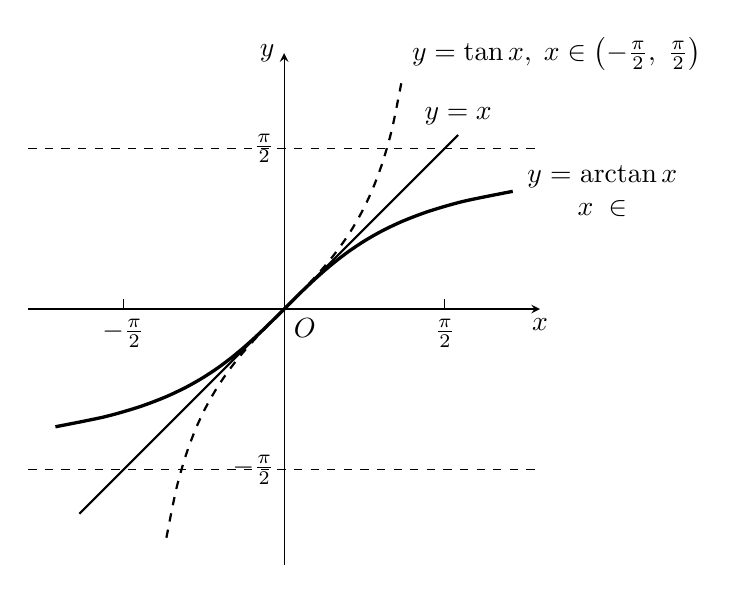
\begin{tikzpicture}[>=stealth, scale=1.3]
    \draw[->](-2.5,0)--(2.5,0)node[below]{$x$};
    \draw[->](0,-2.5)--(0,2.5)node[left]{$y$};
\foreach \x in {pi, -pi}
{
    \draw[dashed](-2.5,\x/2)--(2.5,\x/2);
}
\node at (0,-pi/2)[left]{$-\frac{\pi}{2}$};
\node at (0,pi/2)[left]{$\frac{\pi}{2}$};
\draw(-pi/2,0)node[below]{$-\frac{\pi}{2}$}--(-pi/2,.1);
\draw(pi/2,0)node[below]{$\frac{\pi}{2}$}--(pi/2,.1);
\node [below right]{$O$};
\draw[domain=-1.15:1.15, smooth, thick, dashed]plot(\x, {tan(\x r)})node[above right]{$y=\tan x, \; x\in\left(-\frac{\pi}{2},\; \frac{\pi}{2}\right)$};
\draw[domain=-1.15:1.15, smooth, very thick]plot({tan(\x r)}, \x)node[right, text width=2cm, align=center]{$y=\arctan x$\\ $x\in\R$};
\draw[thick](-2,-2)--(1.7,1.7)node[above]{$y=x$};

\end{tikzpicture}
    \caption{}
\end{figure}

2.反余切函数
\begin{thm}
 {定义4}函数$y=\cot x\; (x\in(0,\pi))$的反函数叫做\textbf{反余切函数},记作$y=\arccot x$,它的定义域是$(-\infty,\infty)$,值域是$(0,\pi)$.   
\end{thm}

反余切函数的图象:见图4.8。

反余切函数的性质:
\begin{enumerate}[(1)]
    \item 对应法则的基本性质:
\begin{enumerate}
    \item $(\arccot x)=x$,其中$x\in\R$.
    \item 当$\alpha\in(0,\pi)$时,$\arccot(\cot\alpha)=\alpha$;当$\alpha\notin(0,\pi)$时,$\arccot(\cot\alpha)\ne\alpha$.
\end{enumerate}
\item 单调性:反余切函数$y=\arccot x$在$(-\infty,\infty)$上是减函数。
\item 奇偶性:反余切函数$y=\arccot x$是非奇非偶函数。
\end{enumerate}


\begin{figure}[htp]
    \centering
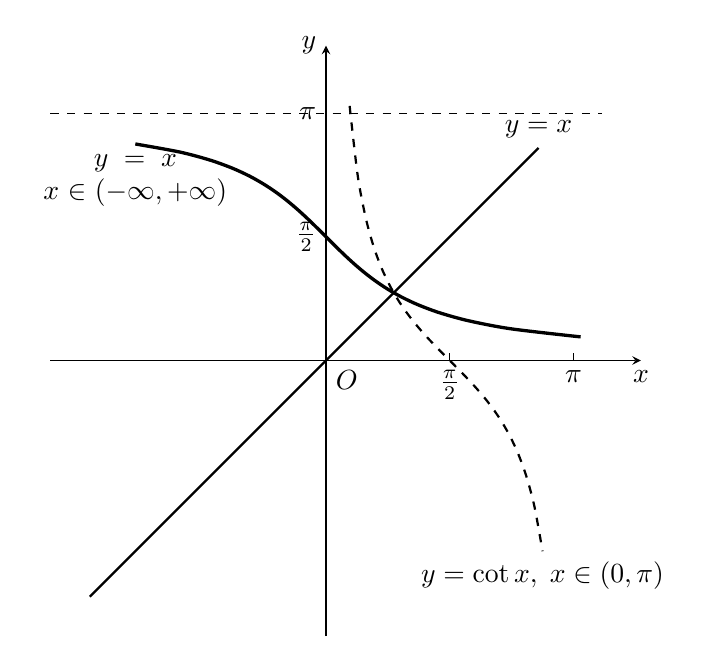
\begin{tikzpicture}[>=stealth, scale=1]
    \draw[->](-3.5,0)--(4,0)node[below]{$x$};
    \draw[->](0,-3.5)--(0,4)node[left]{$y$};
    \draw[dashed](-3.5,pi)--(3.5,pi);
\node at (0,pi/2)[left]{$\frac{\pi}{2}$};
\node at (0,pi)[left]{$\pi$};
\draw(pi/2,0)node[below]{$\frac{\pi}{2}$}--(pi/2,.1);
\draw(pi,0)node[below]{$\pi$}--(pi,.1);
\node [below right]{$O$};
\draw[domain=0.3:2.75, smooth, thick, dashed]plot(\x, {1/tan(\x r)})node[below]{$y=\cot x, \; x\in (0,\pi)$};
\draw[domain=.3:2.75, smooth, very thick]plot({1/tan(\x r)}, \x)node[below, text width=2.5cm, align=center]{$y=\arccot x$\\ $x\in(-\infty,+\infty)$};
\draw[thick](-3,-3)--(2.7,2.7)node[above]{$y=x$};

\end{tikzpicture}
    \caption{}
\end{figure}

反余切函数有下述关系:
\[\arccot(-x)=\pi-\arccot x,\quad x\in(-\infty,\infty)\]

这一点,从图4.9可以看出。

\begin{figure}[htp]
    \centering
\begin{tikzpicture}[>=stealth, scale=1.3]
\draw[->](-2.5,0)--(2.5,0)node[below]{$x$};
\draw[->](0,-1)--(0,2.5)node[left]{$y$};
\draw(1.5,0)node [below]{$A$} arc(0:180:1.5)node[above left]{$\pi$};
\foreach \x in {1.5,-1.5}
{
    \draw[fill=white](\x,0) circle (1.5pt);
}

\draw[dashed](45:1.5*1.414)node[above]{$x$}--(0,0)node[below left]{$O$}--(90+45:1.5*1.414)node[above]{$-x$};
\draw[<->, very thick](45:1.5*1.414)--(90+45:1.5*1.414);
\draw(-2.5,1.5)--(0,1.5)node[above right]{$G$}--(2.5,1.5)node[right]{余切轴};
\node at (45:1.5)[ right]{$P$};
\node at (45+90:1.5)[ left]{$P'$};
\draw[->](.35,0) arc (0:45:.35)node[right]{$\alpha$};
\draw[->](.25,0) arc (0:45+90:.25)node[above]{$\pi-\alpha$};


\end{tikzpicture}
    \caption{}
\end{figure}


\begin{thm}
    {思考题} 证明:$\arccot(-x)=\pi-\arccot x,\quad x\in (-\infty,\infty)$
\end{thm}

反正弦函数、反余弦函数、反正切函数、反余切函数,统称\textbf{反三角函数}\footnote{反三角函数还有反正割函数和反余割函数两种。}。



\begin{example}
    求下列各式的值:
\begin{multicols}{2}
\begin{enumerate}[(1)]
    \item $\arctan1 $
    \item $\arctan\left(-\frac{\sqrt{3}}{3}\right) $
    \item $\arccot0 $
    \item $\arccot\left(-\sqrt{3}\right) $
\end{enumerate}
\end{multicols}
\end{example}

\begin{solution}
\begin{enumerate}[(1)]
    \item $\arctan1 =\frac{\pi}{4}$
    \item $\arctan\left(-\frac{\sqrt{3}}{3}\right)=-\arctan\frac{\sqrt{3}}{3}=-\frac{\pi}{6} $
    \item $\arccot0 =\frac{\pi}{2}$
    \item $\arccot\left(-\sqrt{3}\right) =\pi-\arccot\sqrt{3}=\pi-\frac{\pi}{6}=\frac{5\pi}{6}$
\end{enumerate}    
\end{solution}

\begin{remark}
当$m<0$时,$\arcsin m$、$\arccos m$、$\arctan m$、$\arccot m$的求值,可利用反三角函数的奇偶性或有关公式,化归为$m>0$的情况。
\end{remark}

\begin{example}
    求下列各式的值:
\begin{multicols}{2}
\begin{enumerate}[(1)]
    \item $\tan(\arctan 5)$
    \item $\arctan\left(\tan\frac{2\pi}{3}\right)$
    \item $\arccot\left(\cot\frac{7\pi}{4}\right)$
    \item $\sin[\arctan(-2)]$
\end{enumerate}
\end{multicols}
\end{example}

\begin{solution}
\begin{enumerate}[(1)]
    \item $\tan(\arctan 5)=5$
    \item $\because\quad \frac{2\pi}{3}\notin \left(-\frac{\pi}{2},\; \frac{\pi}{2}\right),\quad \tan\frac{2\pi}{3}=\tan\left(-\frac{\pi}{3}\right)$,而$-\frac{\pi}{3}\in\left(-\frac{\pi}{2},\; \frac{\pi}{2}\right)$

$\therefore\quad \arctan\left(\tan\frac{2\pi}{3}\right)=\arctan \left[\tan\left(-\frac{\pi}{3}\right)\right]=-\frac{\pi}{3}$
    
\item $\because\quad \frac{7\pi}{4}\notin (0,\pi),\quad \cot\frac{7\pi}{4}=\cot\frac{3\pi}{4}$

$\therefore\quad \arccot\left(\cot\frac{7\pi}{4}\right)=\arccot\left(\cot\frac{3\pi}{4}\right)=\frac{3\pi}{4}$

\item 设$\alpha=\arctan (-2)$,则$\tan\alpha=-2$,且$\alpha\in\left(-\frac{\pi}{2},0\right)$,$\sin\alpha=-\frac{1}{\sqrt{5}}$

$\therefore\quad \sin[\arctan(-2)]=\sin\alpha=-\frac{\sqrt{5}}{5}$
\end{enumerate}    
\end{solution}


\begin{example}
求证:$\arctan x+\arccot x=\frac{\pi}{2}$
\end{example}

\begin{analyze}
等式左边复杂,此时往往证明其等价命题$\arctan x=\frac{\pi}{2}-\arccot x$
\end{analyze}

\begin{proof}
\textbf{证法1:}$\tan\left(\frac{\pi}{2}-\arccot x\right)=\cot(\arccot x)=x$

$\because\quad 0<\arccot x<\pi$

$\therefore\quad \frac{\pi}{2}-\arccot x\in\left(-\frac{\pi}{2},\; \frac{\pi}{2}\right)$

因此,$\frac{\pi}{2}-\arccot x$是$\left(-\frac{\pi}{2},\; \frac{\pi}{2}\right)$中的一个角,且它的正切等于$x$,于是$\arctan x=\frac{\pi}{2}-\arccot x$

$\therefore\quad \arctan x+  \arccot x=\frac{\pi}{2}$.

\textbf{证法2:} $\tan(\arctan x)=x,\quad \arctan x\in \left(-\frac{\pi}{2},\; \frac{\pi}{2}\right)$
\[\tan\left(\frac{\pi}{2}-\arccot x\right)=\cot(\arccot x)=x\]

$\because\quad \arccot x\in(0,\pi)$

$\therefore\quad \frac{\pi}{2}-\arccot x \in \left(-\frac{\pi}{2},\; \frac{\pi}{2}\right)$

$\therefore\quad \tan(\arctan x)=\tan\left(\frac{\pi}{2}-\arccot x\right)$

根据正切函数在$\left(-\frac{\pi}{2},\; \frac{\pi}{2}\right)$上是单调函数,可得
\[\arctan x=\frac{\pi}{2}-\arccot x\]

$\therefore\quad \arctan x+  \arccot x=\frac{\pi}{2}$.
\end{proof}

\begin{remark}
 证明两个角相等,往往采用证明其三角函数值相等的方法。采用这种方法时,必须保证两个角都在该三角函数的同一个单调区间内。
\end{remark}


\section*{习题三}
\begin{center}
    \bfseries A
\end{center}

\begin{enumerate}
    \item 求下列各式的值: 
\begin{multicols}{2}
\begin{enumerate}[(1)]
    \item $\arctan \frac{\sqrt{3}}{3}$
    \item $\arccot (-1)$
    \item $\arctan 0$
    \item $\arccot \left(-\frac{\sqrt{3}}{3}\right)$
    \item $\tan \left(\arctan\frac{4\pi}{5}\right)$
    \item $\arctan \left(\tan\frac{4\pi}{5}\right)$
    \item $\cot\left[\arccot \left(-\frac{1}{2}\right)\right] $
    \item $\arccot\left[\cot\left(-\frac{1}{2}\right)\right] $
\end{enumerate}
\end{multicols}
    \item 求下列各式的值: 
\begin{multicols}{2}
\begin{enumerate}[(1)]
    \item $\cot\left[\arctan\frac{2}{5}\right] $
    \item $\sin(\arccot 2)$
    \item $\tan\left(\arctan\frac{1}{4}+\arctan\frac{2}{5}\right) $
    \item $\cos[2\arccot (-5)]$
\end{enumerate}
\end{multicols}
\end{enumerate}

\begin{center}
    \bfseries B
\end{center}

\begin{enumerate}\setcounter{enumi}{2}
    \item 求下列函数的定义域、值域:
\begin{multicols}{2}
\begin{enumerate}[(1)]
    \item $y=2\arctan \frac{x}{2}$
    \item $y=\frac{1}{3}\arccot (1-x)$
\end{enumerate}
\end{multicols}

\item 求值:$\arctan\frac{1}{2}+\arctan\frac{1}{3}$
\item 证明:$\arcsin x+\arccos x=\frac{\pi}{2}$,其中$x\in[-1,1]$.

\end{enumerate}


\section{本章小结}

\subsection{知识结构分析}
四个反三角函数从建立到性质的讨论,都是在反函数一般理论和方法的指导下进行的。为便于对比,也为了使知识
系统化,我们把这四个反三角函数的主要结 论整理 成表如下:


















































































































































\subsection{几点说明}
\begin{enumerate}
\item 反三角函数的建立及注意的问题:

由于确定四个三角函数的映射不是一一映射,所以它们都不存在反函数。我们以三角函数为原型,取它们定义域的子集及其映射,这时它们的映射是一一映射,存在反函数。由此,我们分别定义了四个反三角函数。正因此,我们在研究有关反三角函数的问题时,特别要注意自变量的取值范围。
\item 研究反三角函数的一般方法:

研究反三角函数的性质时,要数形结合,充分利用反三角函数的图象;有时利用三角函数线也是比较 直观和方便的。在解决有关反三角函数的问题时,把问题转化为三角函数的问题,是基本的方法。
\end{enumerate}

\section*{复习题四}

\begin{center}
\bfseries A
\end{center}

\begin{enumerate}
    \item 求下列函数的反函数,并写出反函数的定义域、值域:
\begin{multicols}{2}
\begin{enumerate}[(1)]
    \item $y=2\arccos\frac{x}{4}$
    \item $y=\frac{\pi}{2}+\arctan 2x$
    \item $y=\sin x\quad \left(\frac{\pi}{2}\le x\le \frac{3\pi}{2}\right)$
    \item $y=\cos x\quad \left(-\frac{\pi}{2}\le x\le 0\right)$
\end{enumerate}
\end{multicols}

\item 比较下列各组中两实数的大小:
\begin{multicols}{2}
\begin{enumerate}[(1)]
    \item $\arccos\left(-\frac{7}{8}\right)$与$\arccos\left(-\frac{6}{7}\right)$
    \item $\arctan\left(-3\right)$与$\arctan\left(-5\right)$
    \item $\arcsin\left(\cos 4\right)$与$\arcsin\left(\cos 6\right)$
    \item $\arccot\left(\tan 6\right)$与$\arccot\left(\tan {7}\right)$
\end{enumerate}
\end{multicols}

\item 用反三角中的锐角把下列各式中的$x$表示出来。
\begin{multicols}{2}
\begin{enumerate}[(1)]
    \item $\sin x=-\frac{1}{4}\quad \left(-\frac{\pi}{4}<x<0\right)$
    \item $\sin x=\frac{3}{5}\quad \left(\frac{\pi}{2}<x<\pi\right)$
    \item $\cos x-\frac{3}{7}=0\quad \left(-\frac{\pi}{2}<x<0\right)$
    \item $\cos x=\frac{2}{3}\quad \left(2\pi<x<3\pi\right)$
    \item $\tan x+\sqrt{5}=0\quad \left(\frac{\pi}{2}<x<\pi\right)$
    \item $3\cot x+1=0\quad \left(0<x<\pi\right)$
\end{enumerate}
\end{multicols}

\item 求下列各式的值:
\begin{multicols}{2}
\begin{enumerate}[(1)]
    \item $\sin\left(2\arcsin \frac{1}{4}\right)$
    \item $\cos\left[\frac{1}{2}\arcsin \left(-\frac{4}{5}\right)\right]$
    \item $\cos\left(\arccos\frac{3}{5}-\arcsin\frac{5}{13} \right)$
    \item $\tan\left(\arcsin \frac{3}{5}-\arccos\frac{1}{2}\right)$
\end{enumerate}
\end{multicols}

\item 求下列各式中的$x$:
\begin{multicols}{2}
\begin{enumerate}[(1)]
    \item $\arcsin\frac{20}{29}=\arccos x$
    \item $\arcsin x=\arccos\frac{5}{12}$
    \item $\arccot\frac{11}{60}+\arctan x=0$
\end{enumerate}
\end{multicols}

\item 求下列各式的值:
\begin{multicols}{2}
\begin{enumerate}[(1)]
\item $\arcsin\frac{4}{5}+\arcsin\frac{3}{5}$
\item $\arccos\frac{1}{3}+\arccos\left(-\frac{1}{3}\right)$
\item $\arccot\frac{4}{7}+\arccot \frac{3}{11}$
\item $\arctan\sqrt{3}+\arctan\sqrt{2}$
\end{enumerate}
\end{multicols}

\item 求证下列各式:
\begin{enumerate}[(1)]
    \item $\arcsin x+\arccos x=\frac{\pi}{2}\quad (|x|\le 1)$
    \item $\arctan 1+\arctan 2+\arctan 3=\pi$
\end{enumerate}

\item 已知等腰三角形的高与底的比为$4:3$,用反三角函数把它的三个内角表示出来。
\item 若$m$、$n$为方程$6x^2-5x+1=0$的两个根,

证明:$\arctan m+\arctan n=\frac{\pi}{4}$
\end{enumerate}


\begin{center}
    \bfseries B
\end{center}

\begin{enumerate}\setcounter{enumi}{9}
    \item 求下列函数的定义域、值域:
\begin{multicols}{2}
\begin{enumerate}[(1)]
    \item $y=\frac{1}{\arccos x}$
    \item $y=\arctan\sqrt{x}$
    \item $y=\sqrt{\arctan x}$
    \item $y=\sqrt{\arccot(2x-5)}$
    \item $y=\sqrt{\arcsin\frac{1}{x}}$
    \item $y=\arccos(x^2+x)$
    \item $y=\arccos(\arcsin x)$
    \item $y=\log_a\left(\arccos x-\frac{\pi}{3}\right)$
\end{enumerate}
\end{multicols}


\item 判断函数$y=\arccos x-\frac{\pi}{2}$的奇偶性。
\item 求满足下列不等式的$x$的取值范围;
\begin{multicols}{2}
\begin{enumerate}[(1)]
    \item $\arcsin (-x)<\arcsin x$
    \item $\arccos x<\arccos (1-x)$
\end{enumerate}
\end{multicols}

\end{enumerate}


